\usepackage{amsmath,amsfonts,amsthm,stmaryrd}

\usepackage{xspace}
\usepackage{MnSymbol}
\usepackage[shortlabels,inline]{enumitem}

% \theoremstyle{definition}\newtheorem{definition}{Definition}[section]
% \newtheorem{theorem}[definition]{Theorem}
% \theoremstyle{theorem}\newtheorem{axiom}[definition]{Axiom}
% \theoremstyle{theorem}\newtheorem{lemma}[definition]{Lemma}
% \theoremstyle{theorem}\newtheorem{proposition}[definition]{Proposition}
% \theoremstyle{theorem}\newtheorem{corollary}[definition]{Corollary}
% \theoremstyle{example}\newtheorem{example}[definition]{Example}
\usepackage{hyperref}



\usepackage{tikz}
\usetikzlibrary{arrows.meta}
\def\myarrowhead{Stealth[length=0.8ex,width=0.8ex]}
\tikzset{myarrow/.style={line width=0.1ex}}

\DeclareRobustCommand\myarrowvar{%
  \mathrel{%
    \mbox{$
            \begin{tikzpicture}[baseline=-0.6ex]
                \draw [myarrow, {-\myarrowhead}]
                    (0, 0) -- (2.0ex, 0);
            \end{tikzpicture}%
          $}%
          }
        }

\DeclareRobustCommand\myarrow{%
  \mathrel{%
    \mbox{$
            \begin{tikzpicture}[baseline=-0.6ex]
                \draw [myarrow, {-\myarrowhead}]
                    (0, 0) -- (2.0ex, 0);
            \end{tikzpicture}%
          $}%
          }
        }
\DeclareRobustCommand\mypararrow{%
  \mathrel{%
    \mbox{$
            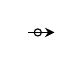
\begin{tikzpicture}[baseline=-0.6ex]
                \draw [myarrow, {-\myarrowhead}]
                (0, 0) -- (2.2ex, 0);
                \draw (0.8ex,0) circle (0.3ex);
            \end{tikzpicture}%
          $}%
          }
}

\DeclareRobustCommand\myleftarrow{%
  \mathrel{%
    \mbox{$
            \begin{tikzpicture}[baseline=-0.6ex]
                \draw [myarrow, {\myarrowhead-}]
                    (0, 0) -- (2.0ex, 0);
            \end{tikzpicture}%
          $}%
          }
}

\DeclareRobustCommand\myleftrightarrow{%
  \mathrel{%
    \mbox{$
            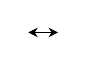
\begin{tikzpicture}[baseline=-0.6ex]
                \draw [myarrow, {\myarrowhead-\myarrowhead}]
                    (0, 0) -- (2.5ex, 0);
            \end{tikzpicture}%
          $}%
          }
}


\newcommand{\gdtt}{\ensuremath{\sym{GDTT}}\xspace}
\newcommand{\gctt}{\ensuremath{\sym{GCTT}}\xspace}
\newcommand{\modalfrp}{\ensuremath{\sym{ModalFRP}}\xspace}

\newcommand\bnfeq{::=}
\newcommand\kleq{\simeq}%kleene equality
\newcommand\sym[1]{\mathsf{#1}}
\newcommand\fix[1]{\sym{fix}^{#1}}
\newcommand\dfix[1][\kappa]{\sym{dfix}^{#1}}
\newcommand\nxt[1][\kappa]{\sym{next}^{#1}}
\newcommand\tabs[2]{\lambda (#1 : #2).}
\newcommand\tickc{\diamond}
%anonymous tick
\newcommand\tick[1][\rho]{
\ooalign{$\checkmark$\cr$^#1$\hss}}
\newcommand\tickA{\alpha}
\newcommand\tickB{\beta}
\newcommand\tapp[2][\tickA]{#2\ [#1] }
\newcommand\tappc[1]{\tapp[\tickc]{#1}}
\newcommand\adv[1][]{\sym{adv}^{#1}}
\newcommand\delay[1][]{\sym{delay}^{#1}}
\newcommand\rbox[1][]{\sym{box}^{#1}}
\newcommand\unbox[1][]{\sym{unbox}^{#1}}
\newcommand\vinterp[2][\rho_E,\rho_N]{\mathcal{V}\llbracket #2 \rrbracket_{#1}}
\newcommand\einterp[2][\rho_E,\rho_N]{\mathcal{E}\llbracket #2 \rrbracket_{#1}}
\newcommand\frplat[1][]{\ensuremath{{\bigcirc}^{#1}}}
\newcommand\frpbox[1][]{\ensuremath{{\Box}^{#1}}}
\newcommand\unlock{\CheckedBox}
\newcommand\open[1]{\sym{open} \; #1}
\newcommand\shut[1]{\sym{shut} \; #1}
\newcommand\push[1]{\sym{push} \; #1}
\newcommand\pull[1]{\sym{pull} \; #1}

%\newcommand\foldI[1][F]{\sym{fold}_{\foldT}}
% \newcommand\fold[1]{\sym{fold}_{#1}}
%\def\foldT{#1}
%\foldI
%}
% \newcommand\foldc{\fold}
%\newcommand\unfoldI[1][F]{\sym{unfold}_{\unfoldT}}
% \newcommand\unfold[1]{\sym{unfold}_{#1}}
%\def\unfoldT{#1}
%\unfoldI
%}
% \newcommand\unfoldc{\unfold[{\tickc}]}

\newcommand\eqmodcl{\approx}

\newcommand\refrule[1]{\textsc{#1}}

\newcommand\defeq{\mathrel{:=}}


\newcommand\sat{\ensuremath{\mathsf{Sat}}\xspace}

\newcommand\ds[1]{\left[#1\right]}
\newcommand\bind[2]{#1\leftarrow #2}
\newcommand\dss[2]{\ds{#1}_{#2}}
\newcommand\prev[1][\kappa]{\sym{prev}{#1}.}
\newcommand\app[1][\kappa]{\mathrel{\circledast^{#1}}}
\newcommand\fv[1]{\sym{fv}(#1)}
\newcommand\ft[1]{\sym{ft}(#1)}
\newcommand\ftc[1]{\sym{ft}^*(#1)}
\newcommand\fc[1]{\sym{fc}(#1)}
\newcommand\bv[1]{\sym{bv}(#1)}
\newcommand\bc[1]{\sym{bc}(#1)}

\newcommand\disj{\mathrel{\#}}


\newcommand\kripke{\ensuremath{{\mathcal K}}\xspace}

\newcommand\pair[2]{\left\langle#1,#2\right\rangle}

\newcommand\clockc{\kappa_0}
\newcommand{\clockkind}{{\small{\sym{c}}}}
\newcommand{\grclock}{{\small{\sym{grclock}}}}
\newcommand{\frpclock}{\sym{frpclock}}
\newcommand{\Fix}{\sym{Fix}\,}
\newcommand{\interm}{\sym{in}}
\newcommand{\caseterm}[5]{\sym{case}\, #1 \, \sym{of}\, \interm_1(#2) . #3 ; \interm_2(#4) . #5}
\newcommand{\letterm}[3]{\sym{let}\, #1 \, = #2 \, \sym{in} \, #3}
\newcommand{\commfp}{\sym{comm}_{\forall,+}}
\newcommand{\stream}[1]{S_{\frplat}^\kappa (#1)}
\newcommand{\gstream}[1]{S^\kappa (#1)}
\newcommand{\rstream}[1]{S_{\frplat} (#1)}


\newcommand\nats{{\mathbb N}}
\newcommand\Str{\sym{Str}}
\newcommand\gStr[1][\kappa]{\sym{Str}^{#1}}
\newcommand\fStrI[1][\kappa]{\sym{Str}^{#1}_{\fStrL}}
\newcommand\fStr[1][\tickA]{
\def\fStrL{#1}
\fStrI
}
\newcommand\gcons[1][\kappa]{\sym{cons}^{#1}}
\newcommand\gconst[1][\kappa]{\sym{const}^{#1}}
\newcommand\gtl[1][\kappa]{\sym{tl}^{#1}}
\newcommand\ghd[1][\kappa]{\sym{hd}^{#1}}
\newcommand\cons{\sym{cons}}
\newcommand\const{\sym{const}}
\newcommand\tl{\sym{tl}}
\newcommand\hd{\sym{hd}}
\newcommand\nth{\sym{nth}}
\newcommand\Nat{\sym{Nat}}
% \newcommand{\latkap}[1]{foooooooooo}
\newcommand\latkap[1][\kappa]{\ensuremath{{\rhd}^{#1}}}
\newcommand\later{\ensuremath{\ \rhd\hspace{-0.3em}}}
\newcommand\latbind[2]{{\rhd}\, (#1:#2) .}
\newcommand\clat[1][\kappa]{\ensuremath{{\hat\rhd}^{#1}}}
\newcommand\clater{\ensuremath{{\hat\rhd}}}
\newcommand\clatbind[2]{\hat{\rhd}\, (#1:#2) .}
\newcommand\ctimes{\mathrel{\hat\times}}
\newcommand\cto{\mathrel{\hat\to}}

\newcommand\Bool{\sym{Bool}}
\renewcommand\tt{\sym{true}}
\newcommand\ff{\sym{false}}
\newcommand\ite{\sym{if}}
\newcommand\suc{\sym{suc}\,}
\newcommand\zero{\sym{0}}
\newcommand\pos[1]{{\mathcal P}os\left(#1\right)}
\newcommand\emptyseq{\langle\rangle}
\newcommand\cat{\cdot}
\newcommand{\id}[0]{\sym{id}}

\newcommand\decr[1]{\left[#1-\right]}

\newcommand\subterm[2]{#1\restriction{#2}}
\newcommand\parto{\rightharpoonup}


\newcommand\injto{\hookrightarrow }

\newcommand\sred{\mathrel{\hat\red}}

\newcommand\red{\myarrow}
\newcommand\redinv{\myleftarrow}
\newcommand\redequiv{\myleftrightarrow^*}
\newcommand\nfred{\red^*_{\mathsf{nf}}}
\newcommand\whred{\red_{\mathsf{WH}}}
\newcommand\whtopred{\mapsto}
\newcommand\whclo[2][\Delta]{#2^{\sym{wh}(#1)}}


\newcommand\CV{\sym{CV}}
\newcommand\TV{\sym{TV}}
\newcommand\Var{\sym{Var}}

\newcommand\pto{\rightharpoonup}
\newcommand\fpowerset[1]{{\mathcal P}_{\mathrm{fin}}(#1)}
\newcommand\subsetfin{\subseteq_{\mathrm{fin}}}

\newcommand\wflab[2][\Delta]{#2 \vdash_{#1}}
\newcommand\wfindex[2][\LL]{#2 \vdash^{#1}}
\newcommand\wfcxt[2][\Delta]{#2 \vdash_{#1}}
\newcommand{\wfclock}[3]{#2\vdash_{#1} #3 \,: \,\sym{clock}}


\newcommand\tokens[1]{\sym{Tok}\left(#1\right)}
\newcommand\weakty[3][\Delta]{#2\vdash_{#1}#3}
\newcommand\type{\sym{type}}
\newcommand\mset[1]{\left\{#1\right\}}
\newcommand\set[1]{\left\{#1\right\}}
\newcommand{\setcom}[2]{\set{#1\left\vert\vphantom{#1}\,#2\right.}}
\newcommand\hastype[4][\Delta]{
#2 \vdash_{#1} #3: #4
}

\newcommand\istype[3][\Delta]{
#2 \vdash_{#1} #3: \type
}

\newcommand\eqtypeII[4][\II]{
#2 \vdash^{\eqtypeL}_{\eqtypeD} #3 \simeq #4:_{#1} \type
}
\newcommand\eqtypeI[1][\LL]{
\def\eqtypeL{#1}
\eqtypeII
}
\newcommand\eqtype[1][\Delta]{
\def\eqtypeD{#1}
\eqtypeI}

\newcommand\sto[4]{{\wfcxt[#1]{#2}} \to {\wfcxt[#3]{#4}}}
\newcommand\subst[2]{\left[#1/#2\right]}
\newcommand\substd[4]{\left[#1/#2,#3/#4\right]}
\newcommand\toksubst[3][\kappa]{\left[#2/#3\right]}
\newcommand\capsubst[2]{\left\{#1/#2\right\}}
\newcommand\substs[3]{\subst{#1}{#2}_{#3}}
\newcommand\repl[2]{\left[#1 \mapsto #2\right]}
\renewcommand\|{\;|\;}


\newcommand\ol[1]{\overline{#1}}

\newcommand{\UU}{{\mathcal U}}
\newcommand\El[1]{\sym{El}\left(#1\right)}

\newcommand\DD{{\mathcal D}}
\newcommand\KK{{\mathcal K}}
\newcommand\LL{{\mathcal L}}
\newcommand\II{{\mathcal I}}
\newcommand\JJ{{\mathcal J}}
\newcommand\TT{{\mathcal T}}
\newcommand\OO{{\mathcal O}}
\newcommand\card[1]{\left|#1\right|}


\newcommand\semcxtII[1]{\left\llbracket #1 \vdash_{\semcxtD}
  \right\rrbracket_{\semcxtN}}

\newcommand\semcxt[1][\Delta]{
\def\semcxtD{#1}
\semcxtI
}

\newcommand\semcxtI[1][\sigma,\delta]{
\def\semcxtN{#1}
\semcxtII}


\newcommand\semlab[2]{\left\llbracket #2\right\rrbracket_{#1}}
\newcommand\semnat{{\mathcal N}}


\newcommand\semtyII[1]{\left\llbracket \vdash_{\semtyD} #1
  \right\rrbracket_{\semtyN}}

\newcommand\semty[1][\Delta]{
\def\semtyD{#1}
\semtyI
}


\newcommand\semtyI[1][\delta]{
\def\semtyN{#1}
\semtyII}



\newcommand\types{\mathsf{Types}}
\newcommand\dom[1]{\mathsf{dom}\left(#1\right)}
\newcommand\supp[1]{\mathsf{supp}\left(#1\right)}

\newcommand\tyvarmaps[1][\Theta]{\left\llbracket #1 \right\rrbracket}
\newcommand\tyvarmapssubst[2][\Theta]{\llbracket #1,#2 \rrbracket}

\newcommand\SN{\ensuremath{\mathsf{SN}}\xspace}
\newcommand\CSN{\ensuremath{\mathsf{CSN}}\xspace}

\newcommand\neutral{\sym{Neu}}

\newcommand\restr[2]{#1\restriction{#2}}

\newcommand\inl{\sym{inl}}
\newcommand\inr{\sym{inr}}

\newcommand\case{\mathsf{case}}

\newcommand\unit{\langle\rangle}
\newcommand\Unit{\sym{1}}
\newcommand\parred{\mypararrow}
\newcommand\binds[1]{\mathsf{dom}\left(#1\right)}


\newcommand{\comm}[3][red]{{\color{#1}{$\spadesuit$#2: #3}}}
\newcommand{\todo}[1]{\comm{TODO}{#1}}


% gDTT macros

\newcommand{\gdttlat}[3][\kappa]{\rhd^{#1}#2.#3}
\newcommand{\hrt}[1]{\left[ #1 \right]}
\newcommand{\typeeqrel}{\ensuremath{\equiv}}
\newcommand{\pure}[3][\kappa]{\nxt[#1]#2.#3}
\newcommand{\termeqrel}{\ensuremath{\equiv}}
\newcommand{\univcode}[1]{\widehat{#1}}
\newcommand{\gdttlatcode}[1]{\univcode{\rhd}^{#1}}

\newcommand{\dsubst}[5]{\ensuremath{\vdash_{#1} #3 : #4 \overset{#2}{\rightarrowtriangle} #5}}
\newcommand{\emptyctx}{\mathop{\cdot}}
\newcommand{\wftype}[3]{\ensuremath{#2 \vdash_{#1} #3 \, \operatorname{type}}}
\newcommand{\isclock}[2]{\ensuremath{\vdash_{#1} #2}}
\newcommand{\alwaystype}[2]{\ensuremath{\forall{#1}{.#2}}}
\newcommand{\dstocm}[3]{\operatorname{adv}_{#1}^{#2}(#3)}
\newcommand{\ctxmorph}[4]{\ensuremath{#2}}% :_{#1} #3 \to #4}}
\newcommand{\esubst}[2]{[#2/#1]} % explicit subst/ctx morph
\newcommand{\alwaysapp}[2]{\ensuremath{#1\!\left[#2\right]}} % eliminator
\newcommand{\termeq}[5]{\ensuremath{#2 \vdash_{#1} #3 \termeqrel #4 : #5}}
\newcommand{\alwaysterm}[2]{\ensuremath{\Lambda{#1}{.#2}}}
\newcommand{\gdtttrans}[1]{#1^*}

\newcommand\qkeep{\sym{keep}}
\newcommand\qdelete{\sym{delete}}
\newcommand\update[3]{[#1 \mapsto \heap{#2}{#3}]}

\newcommand\heap[2]{\pair{#1}{#2}}


% Comments
\newcommand{\rem}[1]{\textbf{REM} #1}

% for complete-easy inference
\newcommand{\checks}[0]{\mathbin{\textcolor{blue}{⇐}}}
\newcommand{\synths}[0]{\mathbin{\textcolor{red}{⇒}}}
\newcommand{\appsynths}[0]{\mathbin{\textcolor{OliveGreen}{⇒\hspace{-.5em}⇒}}}
\newcommand{\bull}[0]{\mathbin{\textcolor{OliveGreen}{∙}}}
\newcommand{\mathhuge}[1]{\mathlarger{\mathlarger{#1}}}
\newcommand{\subt}[0]{\mathbin{\textcolor{Fuchsia}{\code{<:}}}}
\newcommand{\ahat}[0]{\hat{α}}
\newcommand{\bhat}[0]{\hat{β}}
\newcommand{\instantiateLeft}[0]{\code{:=\raisebox{0.5em}{\hspace{-0.6em}<}}}
\newcommand{\instl}[0]{\mathbin{\textcolor{Fuchsia}{\instantiateLeft}}}

\newcommand{\instantiateRight}[0]{\,\code{{=\raisebox{0.5em}{\hspace{-0.6em}<}}}\hspace{-0.3em}:}
\newcommand{\instr}[0]{\mathbin{\textcolor{Fuchsia}{\instantiateRight}}}

\newcommand{\marker}[0]{{\scriptstyle ▶}}

% for clofrp specification
\newcommand{\stable}[0]{stable}
\newcommand{\patcheck}[0]{\mathbin{\textcolor{Bittersweet}{\swneharpoons}}}
\newcommand{\branchcheck}[0]{\mathbin{\textcolor{Emerald}{\Yleft\hspace{-0.5em}⇐}}}
\newcommand{\checkbranch}[4]{(#1\!:\!#2 ⟶ #3) \branchcheck #4}

\newcommand{\Decl}[0]{}
\newcommand{\rulename}[1]{\textsc{\mbox{\Decl#1}}}
\DeclareDocumentCommand{\afk}{ O{χ} O{} }{α\IfNoValueTF{#2}{}{_{#2}}\!:\!#1}
\DeclareDocumentCommand{\ahatk}{ O{χ} O{} }{\ahat\IfNoValueTF{#2}{}{_{#2}}\!:\!#1}
\DeclareDocumentCommand{\bhatk}{ O{χ} O{} }{\bhat\IfNoValueTF{#2}{}{_{#2}}\!:\!#1}
\newcommand{\hask}{\!:\!}
\newcommand{\karr}{\!\!→\!}
\newcommand{\alphas}[0]{\overrightarrow{α}}
\newcommand{\ahats}[0]{\overrightarrow{\hat{α}}}
\newcommand{\fixx}[0]{\sym{fix}}
\newcommand{\fold}[0]{\sym{fold}}
\newcommand{\unfold}[0]{\sym{unfold}}

\newcommand{\haskind}[0]{⤇}
\newcommand{\branch}[1]{ρ_{#1} ⟶ e_{#1}}
\newcommand{\fmap}[0]{\sym{fmap}}

\newcommand{\primRec}[0]{\sym{primRec}}
\newcommand{\alt}[0]{\,|\,}
\newcommand{\Strk}[0]{\textsf{Str}^κ}
\newcommand{\Strka}[0]{\textsf{Str}^κ_α}
\newcommand{\kind}[0]{\chi}
\newcommand{\clockk}[0]{\mathsf{c}}
\newcommand{\Type}[0]{\mathscr{T}}
\newcommand{\Constr}[0]{\mathscr{C}}
\newcommand{\Pat}[0]{\mathscr{P}}
\newcommand{\Rec}[0]{\mathsf{Fix}}
\newcommand{\tickabs}[0]{γ}

\newcommand{\eval}[0]{⇓}
\newcommand{\stepsem}[3]{#1 ⊢ #2 \mathbin{\textcolor{blue}{⇓}} #3}
\newcommand{\appsem}[4]{#1 ⊢ #2\; #3 \mathbin{\textcolor{OliveGreen}{⇊}} #4}
\newcommand{\patsem}[4]{#1 ⊢ #2 \mathbin{\textcolor{Bittersweet}{⇂}} #3 ⊣ #4}
\newcommand{\tickop}[0]{⋙}
\newcommand{\ticksem}[3]{#1 ⊢ #2 \mathbin{\textcolor{BrickRed}{\tickop}} #3}
\newcommand{\forceop}[0]{\lightning}
\newcommand{\force}[3]{#1 ⊢ #2 \mathbin{\textcolor{BurntOrange}{\forceop}} #3}
\newcommand{\clos}[3]{λ_{#1}\,#2.\ #3}
\newcommand{\tclos}[3]{γ_{#1}\,#2.\ #3}

\newcommand{\Maybe}[0]{\textsf{Maybe}}
\newcommand{\Nothing}[0]{\textsf{Nothing}}
\newcommand{\Just}[0]{\textsf{Just}}

\newcommand{\RuleForallL}[0]{\textsc{\ensuremath{≤\hspace{-0.3em}∀}L}\xspace}
\newcommand{\RuleArrowI}[0]{\ensuremath{→}\textsc{I}\ensuremath{\synths}\xspace}
\newcommand{\RuleForallApp}[0]{\textsc{\ensuremath{∀}App}\xspace}

\newcommand{\forallt}[0]{\mathsf{forall}}